\section{定积分 II}

\subsection{定积分相关定理}

\begin{theorem}[Holder 不等式]
	设 $f(x), g(x)$ 在 $[a, b]$ 上可积,那么:
	$$
	\ab(\int_a^b f(x) g(x) \dd{x})^2 \le \int_a^b f(x)^2 \dd{x} \int_a^b g(x)^2 \dd{x}
	$$

	\begin{proof}
		可以发现关于 $t$ 的方程
		$$
		\int_a^b \ab(t f(x) + g(x))^2 \dd{x} = t^2 \int_a^b f(x)^2 \dd{x} + 2t \int_a^b f(x) g(x) \dd{x} + \int_a^b g(x)^2 \dd{x} = 0
		$$
		是一定有解的,因此:
		$$
		\Delta = \ab(2 \int_a^b f(x) g(x) \dd{x})^2 - 4 \int_a^b f(x)^2 \dd{x} \int_a^b g(x)^2 \dd{x} \ge 0
		$$
		于是得证。
	\end{proof}
\end{theorem}

\begin{theorem}[积分第一中值定理]
	设 $f(x), g(x)$ 在 $[a, b]$ 上连续且不变号,那么:
	$$
	\exists\,\xi \in [a, b]: \int_a^b f(x) g(x) \dd{x} = f(\xi) \int_a^b g(x) \dd{x}
	$$
	\begin{proof}
		不妨设 $g(x) \ge 0$,那么有 $\int_a^b g(x) \dd{x} \ge 0$。设 $m \le f(x) \le M$。
		$$
		m \int_a^b g(x) \dd x \le \int_a^b f(x) g(x) \dd x \le M \int_a^b g(x) \dd x
		$$
		当 $g(x) = 0$ 时显然成立,否则就有:
		$$
		m \le \frac{\int_a^b f(x) g(x) \dd{x}}{\int_a^b g(x) \dd{x}} \le M
		$$
		根据介值定理,存在 $\xi \in [a, b]$ 使得
		$$
		f(\xi) = \frac{\int_a^b f(x) g(x) \dd{x}}{\int_a^b g(x) \dd{x}}
		$$
		于是得证。
	\end{proof}
\end{theorem}

积分第一中值定理的一个特例是,若函数 $f(x)$ 在 $[a, b]$ 上连续,那么:
$$
\exists\,\xi \in [a, b]: \int_a^b f(x) \dd{x} = f(\xi)(b - a)
$$
对于一般的可积函数 $f(x)$,我们称 $\frac{1}{b - a} \int_a^b f(x) \dd{x}$ 为 $f(x)$ 在 $[a, b]$ 上的平均值。

\begin{theorem}[积分第二中值定理]
	设 $f(x)$ 在 $[a, b]$ 上可积。
	\begin{itemize}
		\item 若 $g(x)$ 在 $[a, b]$ 上单调递减,且 $g(x) \ge 0$,那么:
		$$
		\exists\,\xi \in [a, b]: \int_a^b f(x) g(x) \dd{x} = g(a) \int_a^\xi f(x) \dd{x}
		$$
		\item 若 $g(x)$ 在 $[a, b]$ 上单调递增,且 $g(x) \ge 0$,那么:
		$$
		\exists\,\eta \in [a, b]: \int_a^b f(x) g(x) \dd{x} = g(b) \int_\eta^b f(x) \dd{x}
		$$
	\end{itemize}
\end{theorem}

\begin{theorem}[积分第三中值定理]
	设 $f(x)$ 在 $[a, b]$ 上可积,$g(x)$ 在 $[a, b]$ 上单调,那么:
	$$
	\exists\,\xi \in [a, b]: \int_a^b f(x) g(x) \dd{x} = g(a) \int_a^\xi f(x) + g(b) \int_\xi^b f(x) \dd{x}
	$$
\end{theorem}

\subsection{微积分基本定理}

对于某个在 $[a, b]$ 上可积的函数 $f(t)$,我们考虑函数:
$$
F(x) = \int_a^x f(t) \dd t \quad (x \in [a, b])
$$
那么我们称 $F(x)$ 为变上限积分。我们接下来对这种函数进行探究。

\begin{theorem}
	若 $f(t)$ 在 $[a, b]$ 上可积,那么 $F(x) = \int_a^x f(t) \dd{t}$ 在 $(a, b)$ 上连续。

	\begin{proof}
		我们需要证明,$\lim\limits_{h \to 0} F(x + h) = F(x)$。
		$$
		F(x_0 + h) - F(x_0) = \int_a^{x_0 + h} f(t) \dd{t} - \int_a^{x_0} f(t) \dd{t} = \int_{x_0}^{x_0 + h} f(t) \dd{t}
		$$
		因为 $f(t)$ 在 $[a, b]$ 有界,那么 $|f(t)| \le M$。于是:
		$$
		\ab|\int_{x_0}^{x_0 + h} f(t) \dd{t}| \le \left|\int_{x_0}^{x_0 + h} |f(t)| \dd{t} \right| \le M |h|
		$$
		于是可得 $F(x_0 + h) - F(x_0) \to 0$。
	\end{proof}
\end{theorem}

\begin{theorem}
	若 $f(t)$ 在 $[a, b]$ 上连续,那么 $F(x) = \int_a^x f(t) \dd t$ 在 $[a, b]$ 上可导,且 $F'(x) = f(x)$。那么:
	$$
	\Delta F = F(x + \Delta x) - F(x) = \int_x^{x + \Delta x} f(t) \dd t = f(\xi) \Delta x
	$$
	而 $\Delta x \to 0$ 时显然 $\xi \to x$,因此:
	$$
	F'(x) = \lim_{\Delta x \to 0} \frac{\Delta F}{\Delta x} = f(x)
	$$
\end{theorem}

那么我们立刻就可以得到:

\begin{theorem}[原函数存在定理]
	若 $f(x)$ 在 $[a, b]$ 上连续,那么 $F(x) = \int_a^x f(x) \dd{x}$ 是 $f(x)$ 在 $[a, b]$ 上的一个原函数。
\end{theorem}

因此,初等函数均存在原函数,但是原函数不一定是初等函数。比如 $\int \frac{\sin x}{x} \dd{x}$。

进一步地,我们可以得到一个微积分中最重要的公式:

\begin{theorem}[Newton-Leibniz 公式]
	若 $f(x)$ 在 $[a, b]$ 上可积,且 $f(x)$ 在 $(a, b)$ 上有原函数 $F(x)$,那么:
	$$
	\int_a^b f(x) \dd{x} = F(b) - F(a) = \left. F(x) \right|_a^b
	$$
	\begin{proof}
		根据定积分的定义,对于任意 $[a, b]$ 的划分 $T$,那么 $\lVert T \rVert \to 0$ 时我们有:
		$$
		\begin{aligned}
			F(b) - F(a) & = \sum_{i=1}^n (F_{x_i} - F_{x_{i-1}}) \\
			& = \sum_{i=1}^n f(\xi_i) (x_i - x_{i-1}) \\
			& = \sum_{i=1}^n f(\xi_i) |\Delta_i| \\
			& = \int_a^b f(x) \dd{x}
		\end{aligned}
		$$
	\end{proof}
\end{theorem}

\subsection{作业}

\begin{problem}
	课后习题 6.3.1

	\begin{solution}
		\begin{enumerate}
			\item[\textbf{1)}] 做代换 $x \gets a \sin t$:
			$$
			\begin{aligned}
				\text{原式} & = \int \frac{\dd (a \sin t)}{a^2 \sin^2 t \cdot a \cos t}  = \int \frac{a \cos t \dd{t}}{a^3 \sin^2 t \cos t} \\
				& = \int \frac{\dd t}{a^2 \sin^2 t} = -\frac{1}{a^2} \cot t + C \\
				& = -\frac{1}{a^2} \cot \arcsin \frac{t}{a} + C = -\frac{1}{a} \sqrt{\frac{1}{x^2} - \frac{1}{a^2}} + C
			\end{aligned}
			$$
			\item[\textbf{2)}] 做代换 $x \gets b \tan t$:
			$$
			\begin{aligned}
				\text{原式} & = \int \frac{\dd (b \tan t)}{b^2 \tan^2 t \cdot b \sec t} = \int \frac{b \sec^2 t \dd{t}}{b^3 \tan^2 t \sec t} \\
				& = \frac{1}{b^2} \int \frac{\dd(\sin t)}{\sin^2 t} = -\frac{1}{b^2 \sin t} + C \\
				& = -\frac{1}{b^2 \sin \arctan \frac{x}{b}} + C = -\frac{1}{b} \sqrt{\frac{1}{x^2} + \frac{1}{b^2}} + C
			\end{aligned}
			$$
			\item[\textbf{5)}]
			$$
			\begin{aligned}
				\text{原式} & = \int \frac{\sinh x}{\cosh^2 x - 1} \dd{x} = \int \frac{\dd(\cosh x)}{\cosh^2 x - 1} \\
				& = \ln \ab(\cosh x + \sqrt{\cosh^2 x - 1}) + C
			\end{aligned}
			$$
			\item[\textbf{7)}] 做代换 $x \gets \arctan t$:
			$$
			\begin{aligned}
				\text{原式} & = \int \frac{\dd(\arctan t)}{1 + t} = \int \frac{\dd t}{(1 + t)(1 + t^2)} \\
				& = \frac{1}{2} \int \ab(\frac{1}{1 + t} + \frac{1}{1 + t^2} - \frac{t}{1 + t^2}) \dd{t} \\
				& = \frac{1}{2} \ln (1 + t) + \frac{1}{2} \arctan t - \frac{1}{4} \ln (1 + t^2) + C \\
				& = \frac{1}{2} \ln (1 + \tan x) + \frac{1}{2} x - \frac{1}{4} \ln \sec^2 x + C \\
			\end{aligned}
			$$
			\item[\textbf{9)}]
			$$
			\begin{aligned}
				\text{原式} & = \int \frac{\dd x}{(1 + \sqrt{2} x + x^2)(1 - \sqrt{2} x + x^2)} \\
				& = \frac{1}{2} \int \ab(\frac{1 - \frac{1}{\sqrt{2}} x}{1 - \sqrt{2} x + x^2} - \frac{1 + \frac{1}{\sqrt{2}} x}{1 + \sqrt{2} x + x^2}) \dd{x} \\
				& = \frac{1}{4 \sqrt{2}} \Big(2 \arctan\ab(1 + \sqrt{2} x) - 2 \arctan\ab(1 - \sqrt{2} x) \\
				& \qquad + \ln\ab(1 + \sqrt{2} x + x^2) - \ln\ab(1 - \sqrt{2} x + x^2)\Big) + C
			\end{aligned}
			$$
			\item[\textbf{10)}]
			$$
			\begin{aligned}
				\text{原式} & = \int \ab(\frac{1}{x^4} - \frac{1}{x^2} + \frac{1}{1 + x^2}) \dd{x} \\
				& = -\frac{1}{3 x^3} + \frac{1}{x} + \arctan x + C
			\end{aligned}
			$$
			\item[\textbf{12)}]
			$$
			\begin{aligned}
				\text{原式} & = \int \frac{x^4 + 1}{(x^2 + 1)(x^4 - x^2 + 1)} \dd{x} \\
				& = \int \frac{(x^4 - x^2 + 1) + x^2}{(x^2 + 1)(x^4 - x^2 + 1)} \dd{x} \\
				& = \int \frac{\dd x}{x^2 + 1} + \frac{1}{3} \int \frac{\dd (x^3)}{x^6 + 1} \\
				& = \arctan x + \frac{1}{3} \arctan x^3 + C
			\end{aligned}
			$$
		\end{enumerate}
	\end{solution}
\end{problem}

\begin{problem}
	课后习题 6.3.2

	\begin{solution}
		\begin{enumerate}
			\item[\textbf{2)}] 做代换 $u = \tan \frac{x}{2}$:
			$$
			\begin{aligned}
				\text{原式} & = \int \frac{\dd(2 \arctan u)}{2 + \frac{2u}{1 + u^2}}= \int \frac{\frac{2}{1 + u^2}}{2 + \frac{2u}{1 + u^2}} \dd{u} \\
				& = \int \frac{\dd u}{(1 + u^2)} = -\frac{1}{1 + u} + C \\
				& = -\frac{1}{1 + 2 \arctan u} + C
			\end{aligned}
			$$

			\item[\textbf{4)}]
			$$
			\text{原式} = \int \frac{x}{x^2 \sqrt{x^2 - 1}} \dd{x} + \int \frac{\dd x}{x^2 \sqrt{x^2 - 1}}
			$$
			其中:
			$$
			\begin{aligned}
				\int \frac{x}{x^2 \sqrt{x^2 - 1}} \dd{x} & = \frac{1}{2} \int \frac{\dd (x^2)}{x^2 \sqrt{x^2 - 1}} \\
				& = \frac{1}{2} \int \frac{\dd (u^2 + 1)}{u (u^2 + 1)} = \int \frac{\dd u}{u^2 + 1} \\
				& = \arctan u + C = \arctan \sqrt{x^2 - 1} + C
			\end{aligned}
			$$
			对于另一项,代换 $x \gets \csc t$:
			$$
			\begin{aligned}
				\int \frac{1}{x^2 \sqrt{x^2 - 1}} & = \int \frac{\dd(\csc t)}{\csc^2 t \cot t} \\
				& = \int \frac{-\cot t \csc t}{\csc^2 t \cot t} \dd{t} = -\int \sin t \dd{t} \\
				& = \cos t + C = \sqrt{1 - \frac{1}{x^2}} + C
			\end{aligned}
			$$
			因此:
			$$
			\text{原式} = \arctan \sqrt{x^2 - 1} + \sqrt{1 - \frac{1}{x^2}} + C
			$$
		\end{enumerate}
	\end{solution}
\end{problem}

\begin{problem}
	课后习题 7.1.1

	\begin{solution}
		\begin{enumerate}
			\item[\textbf{2)}] 我们取划分 $T = \ab\{\frac{1}{n}, \frac{2}{n}, \ldots, \frac{n-1}{n}, 1\},\ \xi_i = \frac{i}{n}$,那么:
			$$
			\begin{aligned}
				\int_0^1 x \dd{x} & = \lim_{n \to \infty} \sum_{i=1}^n \frac{i}{n} \cdot \frac{1}{n} \\
				& = \lim_{n \to \infty} \frac{1}{n^2} \sum_{i=1}^n i \\
				& = \lim_{n \to \infty} \frac{1}{n^2} \cdot \frac{n(n+1)}{2} \\
				& = \lim_{n \to \infty} \frac{n + 1}{2 n} = \frac{1}{2}
			\end{aligned}
			$$

			\item[\textbf{3)}] 记 $L = b - a$,我们取划分 $T = \ab\{a + \frac{L}{n}, a + \frac{2L}{n}, \dots, a + \frac{(n-1)L}{n}, a + L\},\ \xi_i = a + \frac{iL}{n}$,那么:
			$$
			\begin{aligned}
				\int_a^b \frac{\dd x}{x^2} & = \lim_{n \to \infty} \sum_{i=1}^n \frac{1}{\ab(a + \frac{iL}{n})^2} \cdot \frac{L}{n} \\
				& = \lim_{n \to \infty} \frac{L}{n} \sum_{i=1}^n \frac{1}{\ab(a + \frac{iL}{n})^2}
			\end{aligned}
			$$
			而我们有:
			$$
			\begin{aligned}
				\sum_{i=1}^n \frac{1}{(a + \frac{iL}{n})^2} & \le \sum_{i=1}^n \frac{1}{\ab(a + \frac{(i-1)L}{n}) \ab(a + \frac{iL}{n})} \\
				& = \sum_{i=1}^n \frac{n}{L} \ab(\frac{1}{a + \frac{(i-1)L}{n}} - \frac{1}{a + \frac{iL}{n}}) = \frac{n}{L} \ab(\frac{1}{a} - \frac{1}{a + L}) \\
			\end{aligned}
			$$
			$$
			\begin{aligned}
				\sum_{i=1}^n \frac{1}{(a + \frac{iL}{n})^2} & \ge \sum_{i=1}^n \frac{1}{\ab(a + \frac{iL}{n}) \ab(a + \frac{(i+1)L}{n})} \\
				& = \sum_{i=1}^n \frac{n}{L} \ab(\frac{1}{a + \frac{iL}{n}} - \frac{1}{a + \frac{(i+1)L}{n}}) = \frac{n}{L} \ab(\frac{1}{a + \frac{L}{n}} - \frac{1}{a + L + \frac{L}{n}})
			\end{aligned}
			$$
			因此:
			$$
			\begin{gathered}
				\lim_{n \to \infty} \ab(\frac{1}{a + \frac{L}{n}} - \frac{1}{a + L + \frac{L}{n}}) \le \lim_{n \to \infty} \frac{L}{n} \sum_{i=1}^n \frac{1}{\ab(a + \frac{iL}{n})^2} \le \lim_{n \to \infty} \ab(\frac{1}{a} - \frac{1}{a + L}) \\
				\frac{1}{a} - \frac{1}{a + L} \le \lim_{n \to \infty} \frac{L}{n} \sum_{i=1}^n \frac{1}{\ab(a + \frac{iL}{n})^2} \le \frac{1}{a} - \frac{1}{a + L}
			\end{gathered}
			$$
			从而得到:
			$$
			\int_a^b \frac{\dd x}{x^2} = \frac{1}{a} - \frac{1}{a + L} = \frac{1}{a} - \frac{1}{b}
			$$
		\end{enumerate}
	\end{solution}
\end{problem}

\begin{problem}
	课后习题 7.1.2

	\begin{solution}
		\begin{enumerate}
			\item[\textbf{2)}] 函数的图像如下:
			\begin{figure}[H]
				\centering
				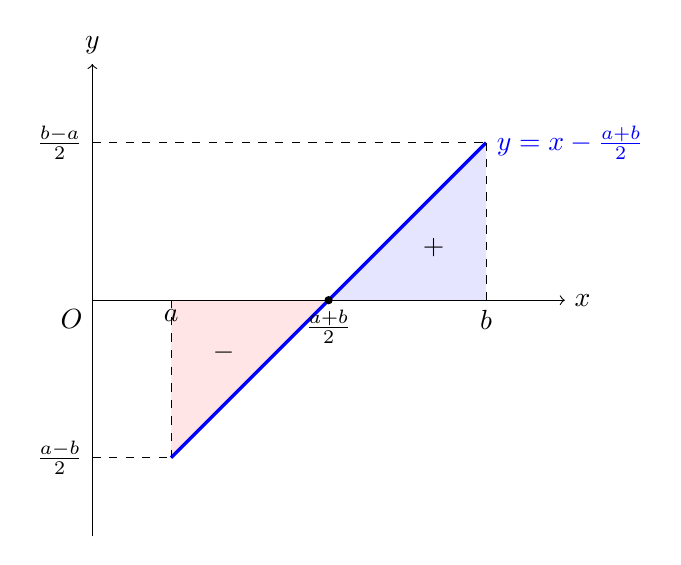
\begin{tikzpicture}
					\pgfmathsetmacro{\aval}{1} % Example value for a
					\pgfmathsetmacro{\bval}{5} % Example value for b
					\pgfmathsetmacro{\midval}{(\aval + \bval) / 2}
					\pgfmathsetmacro{\ya}{\aval - \midval}
					\pgfmathsetmacro{\yb}{\bval - \midval}

					% Fill areas indicating positive and negative regions
					\fill[red!10] (\aval, 0) -- (\aval, \ya) -- (\midval, 0) -- cycle;
					\node at ({(\aval + \aval + \midval)/3}, {\ya/3}) {$-$};

					\fill[blue!10] (\midval, 0) -- (\bval, 0) -- (\bval, \yb) -- cycle;
					\node at ({(\midval + \bval + \bval)/3}, {\yb/3}) {$+$};

					% Axes
					\draw[->] (\aval - 1, 0) -- (\bval + 1, 0) node[right] {$x$};
					\draw[->] (0, \ya - 1) -- (0, \yb + 1) node[above] {$y$};
					\node[below left] at (0,0) {$O$};

					% Plot the function y = x - (a+b)/2
					\draw[very thick, blue, domain=\aval:\bval] plot (\x, {\x - \midval}) node[right] {$y = x - \frac{a+b}{2}$};

					% Mark a and b on the x-axis
					\draw[dashed] (\aval, 0) -- (\aval, {\ya});
					\node[below] at (\aval, 0) {$a$};
					\draw[dashed] (\bval, 0) -- (\bval, {\yb});
					\node[below] at (\bval, 0) {$b$};

					% Mark the y-values at a and b
					\draw[dashed] (0, {\ya}) -- (\aval, {\ya});
					\node[left] at (0, {\ya}) {$\frac{a-b}{2}$};
					\draw[dashed] (0, {\yb}) -- (\bval, {\yb});
					\node[left] at (0, {\yb}) {$\frac{b-a}{2}$};

					% Mark the intercept (a+b)/2 on the x-axis
					\node[below] at (\midval, 0) {$\frac{a+b}{2}$};
					\fill (\midval, 0) circle (1.5pt);

				\end{tikzpicture}
				\caption{函数 $y = x - \frac{a+b}{2}$ 的图像}
			\end{figure}

			根据定积分的几何意义,该积分值为 $0$。
		\end{enumerate}
	\end{solution}
\end{problem}

\begin{problem}
	课后习题 7.2.7

	\begin{solution}
		\begin{enumerate}
			\item[\textbf{2)}] 对于任意 $\varepsilon > 0$:
			$$
			\begin{aligned}
				\int_0^{\frac{\pi}{2}} \sin^n x \dd{x} & = \int_0^{\frac{\pi - \varepsilon}{2}} \sin^n x \dd{x} + \int_{\frac{\pi - \varepsilon}{2}}^{\frac{\pi}{2}} \sin^n x \dd{x} \\
				& \le \ab(\frac{\pi - \varepsilon}{2}) \sin^n \frac{\pi - \varepsilon}{2} + \frac{\varepsilon}{2} \\
				& < \frac{\pi}{2} \sin^n \frac{\pi - \varepsilon}{2} + \frac{\varepsilon}{2}
			\end{aligned}
			$$
			那么,取 $N = \ceil{\frac{\ln \varepsilon / \pi}{\ln \sin \frac{\pi - \varepsilon}{2}}}$,那么当 $n \ge N$ 时,有:
			$$
			\int_0^{\frac{\pi}{2}} \sin^n x \dd{x} < \varepsilon
			$$
			因此得到 $\lim\limits_{n \to 0} \int_0^{\frac{\pi}{2}} \sin^n x \dd{x} = 0$。

			\item[\textbf{4)}]
			$$
			\lim_{n \to \infty} \abs{\int_n^{n+1} \frac{\cos x}{x} \dd{x}} \le \lim_{n \to \infty} \int_n^{n+1} \abs{\frac{\cos x}{x}} \dd{x} \le \lim_{n \to \infty} \abs{\frac{1}{n + 1}} = 0
			$$
			因此
			$$
			\lim_{n \to \infty} \int_n^{n+1} \frac{\cos x}{x} \dd{x} = 0
			$$
		\end{enumerate}
	\end{solution}
\end{problem}

\begin{problem}
	课后习题 7.2.8

	\begin{proof}
		\begin{enumerate}
			\item[\textbf{3)}] 记 $f(x) = \frac{\sin x}{x}$,那么:
			$$
			f'(x) = \frac{x \cos x - \sin x}{x^2}
			$$
			当 $0 < x < \frac{\pi}{2}$ 时,$\tan x > x \Leftrightarrow \sin x > x \cos x$,因此 $f'(x) < 0$,$f(x)$ 单调递减。于是:
			$$
			\begin{gathered}
				f\ab(\frac{\pi}{2}) < \int_0^1 f(x) \dd{x} < f(0) \\
				\frac{2}{\pi} < \int_0^1 f(x) \dd{x} < 1
			\end{gathered}
			$$
		\end{enumerate}
	\end{proof}
\end{problem}

\begin{problem}
	课后习题 7.2.9

	\begin{proof}
		$$
		\begin{aligned}
			& & \int_0^\beta f(x) \dd{x} & \ge \beta \int_0^1 f(x) \dd{x} \\
			\Leftrightarrow & & \int_0^\beta f(x) \dd{x} & \ge \beta \int_0^\beta f(x) \dd{x} + \beta \int_\beta^1 f(x) \dd{x} \\
			\Leftrightarrow & & (1 - \beta) \int_0^\beta f(x) \dd{x} & \ge \beta \int_\beta^1 f(x) \dd{x} \\
			\Leftrightarrow & & \frac{1}{\beta} \int_0^\beta f(x) \dd{x} & \ge \frac{1}{1 - \beta} \int_\beta^a f(x) \dd{x} \\
		\end{aligned}
		$$
		根据积分第一中值定理:
		$$
		\exists\,\xi \in (0, \beta), \exists\,\eta \in (\beta, 1): \frac{1}{\beta} \int_0^\beta f(x) \dd{x} = f(\xi),\ \frac{1}{1 - \beta} \int_\beta^1 f(x) \dd{x} = f(\eta)
		$$
		而 $\xi < \beta < \eta$,因此 $f(\xi) \ge f(\beta)$,于是得证。
	\end{proof}
\end{problem}

\begin{problem}
	课后习题 7.2.10

	\begin{proof}
		\begin{enumerate}
			\item[\textbf{1)}] 设 $A(x) = f(x) \sin x,\ B(x) = g(x) \cos x$。那么即证:
			$$
			\ab(\int_a^b A(x) \dd{x})^2 + \ab(\int_a^b B(x) \dd{x})^2 \le (b - a) \int_a^b \ab(A(x)^2 + B(x)^2) \dd{x}
			$$
			取 $[a, b]$ 的一个等分 $T = \ab\{a + \frac{b - a}{n}, a + \frac{2(b - a)}{n}, \dots, a + \frac{(n - 1)(b - a)}{n}, b\}$,取 $\xi_i = a + \frac{i (b - a)}{n}$,记 $\Delta x = \frac{b - a}{n}$,那么根据柯西不等式有:
			$$
			\begin{gathered}
				\ab(\sum_{i=1}^n A(\xi_i))^2 \le n \sum_{i=1}^n A(\xi_i)^2 \\
				\ab(\sum_{i=1}^n B(\xi_i))^2 \le n \sum_{i=1}^n B(\xi_i)^2
			\end{gathered}
			$$
			将两式相加,两侧乘上 $\Delta x^2$,那么得到:
			$$
			\ab(\sum_{i=1}^n A(\xi_i) \Delta x)^2 + \ab(\sum_{i=1}^n B(\xi_i) \Delta x)^2 \le (b - a) \sum_{i=1}^n \ab(A(\xi_i)^2 + B(\xi_i)^2) \Delta x
			$$
			根据极限保号性,我们令 $\Delta x \to 0$,得到:
			$$
			\ab(\int_a^b A(x) \dd{x})^2 + \ab(\int_a^b B(x) \dd{x})^2 \le (b - a) \int_a^b \ab(A(x)^2 + B(x)^2) \dd{x}
			$$

			\item[\textbf{2)}] 取 $[a, b]$ 的一个等分 $T = \ab\{a + \frac{b - a}{n}, a + \frac{2(b - a)}{n}, \dots, a + \frac{(n - 1)(b - a)}{n}, b\}$,记 $a_i = f\ab(a + \frac{i (b - a)}{n})$,那么:
			$$
			\begin{aligned}
				& \ab(\sum_{i=1}^n a_i \sin ni)^2 + \ab(\sum_{i=1}^n a_i \cos ni)^2 - \ab(\sum_{i=1}^n a_i)^2 \\
				= & \sum_{i=1}^n \sum_{j=1}^n a_i a_j \ab(\sin ni \sin nj + \cos ni \cos nj - 1) \\
				= & \sum_{i=1}^n \sum_{j=1}^n a_i a_j \ab(\cos (ni - nj) - 1) \le 0
			\end{aligned}
			$$
			给上式乘上 $\ab(\frac{b - a}{n})^2$,然后根据极限的保号性,令 $n \to \infty$ 就得到:
			$$
			\ab(\int_a^b f(x) \sin nx \dd{x})^2 + \ab(\int_a^b f(x) \cos nx \dd{x})^2 \le \ab(\int_a^b f(x) \dd{x})^2
			$$
		\end{enumerate}
	\end{proof}
\end{problem}